% PVLDB Volume 20 / VLDB 2027 vision paper.
% Category suffix [Vision] is required at submission (dropped in camera-ready).
\documentclass[sigconf, nonacm]{acmart}

%%% do not modify the following VLDB block %%
%%% VLDB block start %%%
\usepackage{pvldb}
%%% VLDB block end %%%

\usepackage{tikz}
\usetikzlibrary{arrows.meta,positioning,fit,calc,shapes.geometric}
\usepackage{booktabs}
\usepackage{array}
\usepackage{microtype}

% Breakable inlines so two-column text cannot spill into the gutter.
\newcommand{\cbras}{\texttt{answer}/\allowbreak\texttt{set}/\allowbreak\texttt{abstain}}
\newcommand{\cbraa}{\texttt{answer}/\allowbreak\texttt{abstain}}
\newcommand{\cbrth}{0.50, 0.70, 0.90, 0.95, and 0.99}
\usepackage{listings}
\lstset{basicstyle=\scriptsize\ttfamily,columns=fullflexible,keepspaces=true,
  frame=single,rulecolor=\color{black!20},aboveskip=4pt,belowskip=4pt,
  xleftmargin=2pt,xrightmargin=2pt,breaklines=true,framexleftmargin=2pt}
% CalibRead vision-paper figures — crisp color palette (print + screen).
\definecolor{cbrblue}{HTML}{2E86AB}
\definecolor{cbrbluefill}{HTML}{E8F4FA}
\definecolor{cbrcoral}{HTML}{E07A5F}
\definecolor{cbrcoralfill}{HTML}{FDEEEA}
\definecolor{cbrgreen}{HTML}{2A9D8F}
\definecolor{cbrgreenfill}{HTML}{E6F6F3}
\definecolor{cbrviolet}{HTML}{5B4FCF}
\definecolor{cbrvioletfill}{HTML}{EEECFA}
\definecolor{cbramber}{HTML}{E9A319}
\definecolor{cbramberfill}{HTML}{FFF6E5}
\definecolor{cbrink}{HTML}{1F2937}
\definecolor{cbrmuted}{HTML}{6B7280}

\tikzset{
  cbr/.style={font=\footnotesize, text=cbrink},
  cbrbox/.style={draw=cbrink!55, rounded corners=3pt, align=center,
    inner sep=6pt, line width=0.55pt, text=cbrink},
  cbrarr/.style={-{Latex[length=2.2mm,width=1.6mm]}, line width=0.65pt, draw=cbrink!70},
  cbrdash/.style={-{Latex[length=2.2mm,width=1.6mm]}, line width=0.65pt, draw=cbrcoral!80, dashed},
  cbrlbl/.style={font=\scriptsize\bfseries, text=cbrmuted, align=center},
}
\newcommand{\cbrtitle}[1]{{\scriptsize\bfseries #1}}

% Figure 1: motivating placement in a hybrid query plan
\newcommand{\CalibReadFigMotivation}{%
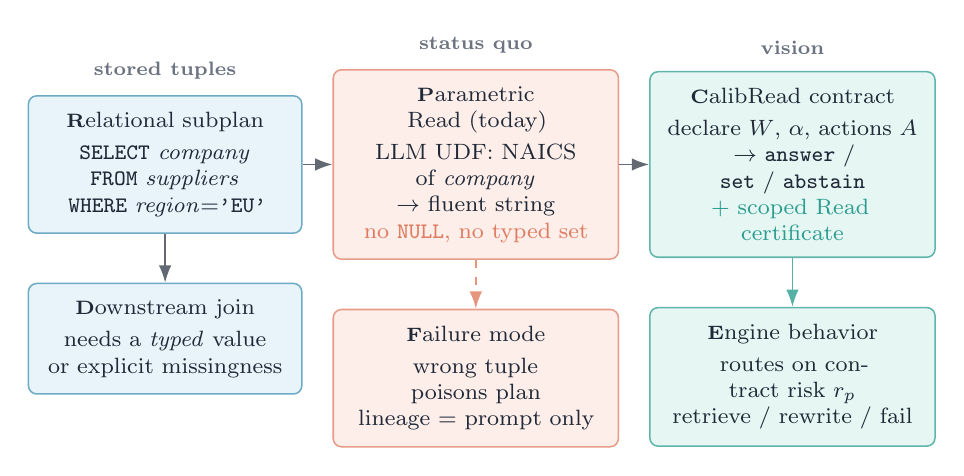
\begin{tikzpicture}[cbr, node distance=0.42cm and 0.38cm]
  \node[cbrbox, fill=cbrbluefill, draw=cbrblue!70, text width=3.05cm] (sql) {%
    {\cbrtitle Relational subplan}\\[2pt]
    \texttt{SELECT} \emph{company}\\
    \texttt{FROM} \emph{suppliers}\\
    \texttt{WHERE} \emph{region}=\texttt{'EU'}};
  \node[cbrlbl, above=0.08cm of sql] {stored tuples};
  \node[cbrbox, fill=cbrcoralfill, draw=cbrcoral!75, text width=3.2cm, right=of sql] (udf) {%
    {\cbrtitle Parametric Read (today)}\\[2pt]
    LLM UDF: {NAICS} of \emph{company}\\
    $\rightarrow$ fluent string\\
    \textcolor{cbrcoral}{no \texttt{NULL}, no typed set}};
  \node[cbrlbl, above=0.08cm of udf] {status quo};
  \node[cbrbox, fill=cbrgreenfill, draw=cbrgreen!75, text width=3.2cm, right=of udf] (cbr) {%
    {\cbrtitle CalibRead contract}\\[2pt]
    declare $W$, $\alpha$, actions $A$\\
    $\rightarrow$ \texttt{answer} / \texttt{set} / \texttt{abstain}\\
    \textcolor{cbrgreen}{+ scoped Read certificate}};
  \node[cbrlbl, above=0.08cm of cbr] {vision};
  \node[cbrbox, fill=cbrbluefill, draw=cbrblue!70, text width=3.05cm, below=0.62cm of sql] (join) {%
    {\cbrtitle Downstream join}\\[2pt]
    needs a \emph{typed} value\\
    or explicit missingness};
  \node[cbrbox, fill=cbrcoralfill, draw=cbrcoral!75, text width=3.2cm, below=0.62cm of udf] (bad) {%
    {\cbrtitle Failure mode}\\[2pt]
    wrong tuple poisons plan\\
    lineage = prompt only};
  \node[cbrbox, fill=cbrgreenfill, draw=cbrgreen!75, text width=3.2cm, below=0.62cm of cbr] (good) {%
    {\cbrtitle Engine behavior}\\[2pt]
    routes on contract risk $r_p$\\
    retrieve / rewrite / fail};
  \draw[cbrarr] (sql) -- (udf);
  \draw[cbrarr] (udf) -- (cbr);
  \draw[cbrarr] (sql) -- (join);
  \draw[cbrdash] (udf) -- (bad);
  \draw[cbrarr, draw=cbrgreen!80] (cbr) -- (good);
\end{tikzpicture}}

% Figure 2: system architecture
\newcommand{\CalibReadFigArchitecture}{%
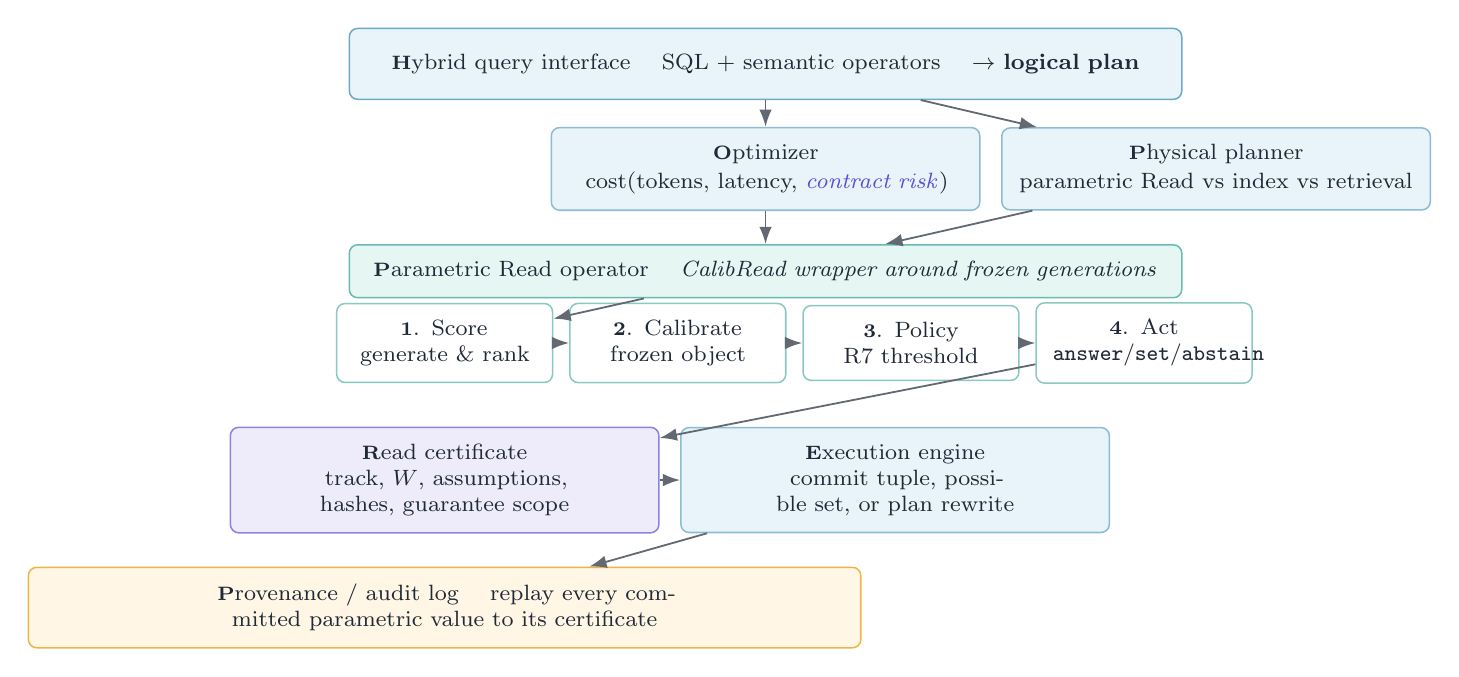
\begin{tikzpicture}[cbr, node distance=0.34cm and 0.26cm]
  \node[cbrbox, fill=cbrbluefill, draw=cbrblue!70, text width=10.15cm, minimum height=0.9cm] (iface) {%
    {\cbrtitle Hybrid query interface} \quad
    SQL + semantic operators \quad $\rightarrow$ \textbf{logical plan}};
  \node[cbrbox, fill=cbrbluefill, draw=cbrblue!55, text width=5.02cm, below=of iface] (opt) {%
    {\cbrtitle Optimizer}\\[1pt]
    cost(tokens, latency, \textcolor{cbrviolet}{\emph{contract risk}})};
  \node[cbrbox, fill=cbrbluefill, draw=cbrblue!55, text width=5.02cm, right=of opt] (phys) {%
    {\cbrtitle Physical planner}\\[1pt]
    parametric Read vs index vs retrieval};
  \node[cbrbox, fill=cbrgreenfill, draw=cbrgreen!70, text width=10.15cm, below=0.42cm of opt] (mod) {%
    {\cbrtitle Parametric Read operator} \quad
    \textit{CalibRead wrapper around frozen generations}};
  \node[cbrbox, fill=white, draw=cbrgreen!55, text width=2.32cm, below=0.4cm of mod.west, xshift=1.22cm] (gen) {%
    {\cbrtitle 1. Score}\\generate \& rank};
  \node[cbrbox, fill=white, draw=cbrgreen!55, text width=2.32cm, right=0.2cm of gen] (cal) {%
    {\cbrtitle 2. Calibrate}\\frozen object};
  \node[cbrbox, fill=white, draw=cbrgreen!55, text width=2.32cm, right=0.2cm of cal] (pol) {%
    {\cbrtitle 3. Policy}\\R7 threshold};
  \node[cbrbox, fill=white, draw=cbrgreen!55, text width=2.32cm, right=0.2cm of pol] (act) {%
    {\cbrtitle 4. Act}\\\texttt{answer}/\texttt{set}/\texttt{abstain}};
  \node[cbrbox, fill=cbrvioletfill, draw=cbrviolet!70, text width=5.02cm, below=0.55cm of gen] (cert) {%
    {\cbrtitle Read certificate}\\track, $W$, assumptions, hashes, guarantee scope};
  \node[cbrbox, fill=cbrbluefill, draw=cbrblue!55, text width=5.02cm, right=of cert] (exec) {%
    {\cbrtitle Execution engine}\\commit tuple, possible set, or plan rewrite};
  \node[cbrbox, fill=cbramberfill, draw=cbramber!80, text width=10.15cm, below=0.42cm of cert] (prov) {%
    {\cbrtitle Provenance / audit log} \quad replay every committed parametric value to its certificate};
  \draw[cbrarr] (iface) -- (opt);
  \draw[cbrarr] (iface) -- (phys);
  \draw[cbrarr] (opt) -- (mod);
  \draw[cbrarr] (phys) -- (mod);
  \draw[cbrarr] (mod) -- (gen);
  \draw[cbrarr] (gen) -- (cal);
  \draw[cbrarr] (cal) -- (pol);
  \draw[cbrarr] (pol) -- (act);
  \draw[cbrarr] (act) -- (cert);
  \draw[cbrarr] (cert) -- (exec);
  \draw[cbrarr] (exec) -- (prov);
\end{tikzpicture}}

% Figure 2: two evaluation tracks (side-by-side columns, clean merge arrows)
\newcommand{\CalibReadFigTracks}{%
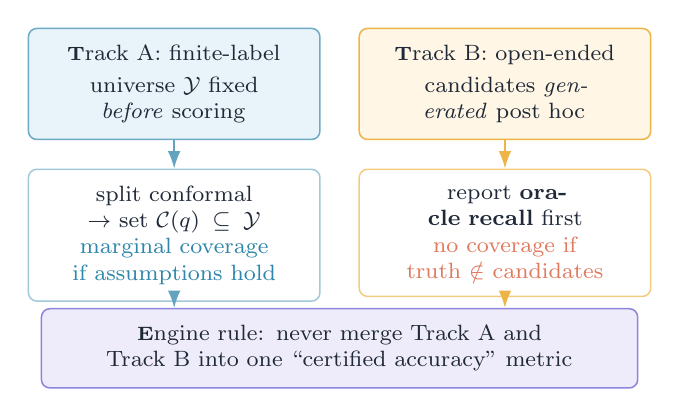
\begin{tikzpicture}[cbr, node distance=0.36cm and 0.48cm]
  \node[cbrbox, fill=cbrbluefill, draw=cbrblue!70, text width=3.28cm] (ta) {%
    {\cbrtitle Track A: finite-label}\\[2pt]
    universe $\mathcal{Y}$ fixed \emph{before} scoring};
  \node[cbrbox, fill=white, draw=cbrblue!45, text width=3.28cm, below=of ta] (taf) {%
    split conformal $\rightarrow$ set $\mathcal{C}(q)\subseteq\mathcal{Y}$\\
    \textcolor{cbrblue}{marginal coverage if assumptions hold}};
  \node[cbrbox, fill=cbramberfill, draw=cbramber!80, text width=3.28cm, right=of ta] (tb) {%
    {\cbrtitle Track B: open-ended}\\[2pt]
    candidates \emph{generated} post hoc};
  \node[cbrbox, fill=white, draw=cbramber!55, text width=3.28cm, below=of tb] (tbf) {%
    report \textbf{oracle recall} first\\
    \textcolor{cbrcoral}{no coverage if truth $\notin$ candidates}};
  \node[cbrbox, fill=cbrvioletfill, draw=cbrviolet!70, text width=7.15cm] (rule) at
    ($(taf.south)!0.5!(tbf.south) + (0,-0.62)$) {%
    {\cbrtitle Engine rule:} never merge Track A and Track B into one ``certified accuracy'' metric};
  \draw[cbrarr, draw=cbrblue!75] (ta.south) -- (taf.north);
  \draw[cbrarr, draw=cbramber!80] (tb.south) -- (tbf.north);
  \draw[cbrarr, draw=cbrblue!75] (taf.south) -- (rule.north -| taf.south);
  \draw[cbrarr, draw=cbramber!80] (tbf.south) -- (rule.north -| tbf.south);
\end{tikzpicture}}


%% Paper-specific PVLDB metadata (placeholders are fine until production).
\renewcommand\vldbdoi{XX.XX/XXX.XX}
\renewcommand\vldbpages{XXX-XXX}
% Vision submission: no experimental artifact package is required if none is claimed.
\renewcommand\vldbavailabilityurl{}

\begin{document}
\title{CalibRead: Reliability Contracts for Parametric LLM Databases [Vision]}
% Used in the mandatory PVLDB Reference Format block (\vldbtopmatter).
\renewcommand\vldbtitle{CalibRead: Reliability Contracts for Parametric LLM Databases [Vision]}

\author{Aadit Shah}
\affiliation{%
  \institution{Birla Institute of Technology and Science, Pilani}
  \city{Pilani}
  \country{India}
}
\email{f20220612@pilani.bits-pilani.ac.in}

\author{Yash Sinha}
\affiliation{%
  \institution{Birla Institute of Technology and Science, Pilani}
  \city{Pilani}
  \country{India}
}
\email{yash.sinha@pilani.bits-pilani.ac.in}

\begin{abstract}
Database engines treat a \emph{Read} as a contract: given a well-formed request, the system returns stored values, reports absence, or signals that the request cannot be answered under the declared isolation, integrity, and completeness assumptions. Large language models (LLMs) are increasingly invoked as parametric stores in hybrid SQL, as operators in semantic query engines, and as oracles for facts missing from tables, yet they return fluent strings with no comparable contract.

\textbf{CalibRead makes reliability an executable property of a parametric query operator}: a typed \cbras{} Read, a scoped certificate $C$ that is why-provenance for the parametric value, and plan-time \emph{contract risk} that the optimizer can cost the way it costs selectivity. The library implements generation, calibration, fail-closed policy, and certificate emission; the SQL operator and planner rewrite are specified, not implemented. Open questions are how certificates compose beyond fail-closed hops, how labeled calibration support is budgeted, how the planner costs $r_p$, and how $C$ is logged.
\end{abstract}

\maketitle

%%% do not modify the following VLDB block %%
%%% VLDB block start %%%
\vldbtopmatter
%%% VLDB block end %%%

\section{Introduction}

The last three years have made an implicit bet: that large language models can stand in for missing tables, missing joins, and missing world knowledge inside data systems. Hybrid querying attaches LLM calls to SQL so that ``beyond-database'' questions become first-class~\cite{zhao2025swan,saeed2023galois}. Semantic operator systems compile natural-language maps, filters, and joins into LLM-backed plans and optimize cost and quality~\cite{patel2025lotus,liu2025palimpzest,russo2026abacus,shankar2025docetl}. Neural databases answer queries over facts supplied as text~\cite{thorpe2021neuraldb}. A parametric Read goes one step further. The fact is in neither a table nor a passage, and the model weights are the store. Commercial engines expose LLM user-defined functions that planners treat as black boxes, so invocation cost never enters the plan~\cite{an2025aidb}. Wherever this happens, the model is used as a \emph{Read}: the application asks for a value and proceeds as if the returned string were data.

That bet fails the oldest test in data management. Under a closed-world or explicitly incomplete interpretation, a relational engine returns the stored value, returns a marked unknown, or refuses the query~\cite{imielinski1984incomplete,abiteboul1991update,dalvi2007efficient,suciu2011probabilistic,widom2005trio}. It will not invent an industry code for a missing supplier, and it will not report a confidence of $0.97$ that is uncorrelated with error in the long tail. LLMs do both~\cite{guo2017calibration,kadavath2022language,kalai2024calibrated}. Nest one of those generators in a query plan and a single hallucinated Read poisons every downstream operator. The lineage, in that case, is a prompt rather than a tuple identifier. On the 120-question SWAN benchmark, few-shot GPT-4 Turbo reaches 40\% execution accuracy~\cite{zhao2025swan}. Parametric Reads are a poor substitute for a drop-in \texttt{SELECT}, which is why they need a contract.

Guardrails have started to appear. Semantic integrity constraints declare grounding, format, and exclusion checks on LLM outputs~\cite{lee2025sic}. LOTUS cascades a cheap proxy against a gold algorithm and guarantees fidelity to that algorithm. Abacus then costs quality, dollars, and latency~\cite{patel2025lotus,russo2026abacus}. Conformal language modeling and conformal factuality wrap generation with set-valued or claim-level guarantees under stated assumptions~\cite{quach2024conformal,mohri2024language,wang2024conu}. SUPG and probabilistic predicates let a processor route an ML operator on a budgeted precision or recall target~\cite{kang2020supg,lu2018probabilistic}. ConRAD allocates a marginal-recall budget across link predictors on a neural knowledge graph and skips inference when the graph already suffices~\cite{horchidan2026conrad}. A parametric \emph{Read} still has to supply what those mechanisms leave open: typed commit versus set versus abstain, a workload-scoped certificate, fail-closed integrity when calibration support is missing, and plan-time contract risk for a generator that may have no scored candidate at all.

\textbf{CalibRead makes reliability an executable property of a parametric query operator, not a statistical property of an LLM prediction.} Adjacent work supplies the pieces (Table~\ref{tab:position}). Integrating them into an execution contract lets a planner choose parametric versus retrieval versus human the way it already chooses an access path.

The contract has three parts: (i)~typed \texttt{answer}, \texttt{set}, or \texttt{abstain} actions; (ii)~workload-conditioned validity over R1--R7 metadata (Section~\ref{sec:surface}); (iii)~auditable scope. Finite-label Reads may inherit \emph{marginal} conformal coverage under exchangeability~\cite{vovk2005algorithmic}. Open-ended generation inherits no set-coverage of the true value. Claim-level factuality is a different statement~\cite{mohri2024language,wang2024conu}. The engine keeps those two validity claims on separate tracks.

\begin{figure*}[t]
  \centering
  \CalibReadFigMotivation
  \caption{Hybrid plans already issue parametric Reads, but today's LLM UDFs return untyped strings. CalibRead turns the Read into a database operator with explicit actions and provenance.}
  \Description{Three-column comparison of a relational subplan feeding a parametric LLM read, contrasting today's fluent-string UDF with a CalibRead contract that returns answer, set, or abstain plus a certificate.}
  \label{fig:motivation}
\end{figure*}

For a supplier whose NAICS class is not in any table, CalibRead may return a singleton code, a set of codes, or \texttt{abstain}. It does not return a silent fluent guess (Figure~\ref{fig:motivation}). The Python library implements the contract of Section~\ref{sec:opsketch}. Listings~\ref{lst:sql}--\ref{lst:rewrite} and planner integration are the agenda~\cite{lee2025sic}.

\begin{table*}[t]
\caption{Novelty is the \emph{execution contract}, not any one mechanism. Each prior line remains a component CalibRead consumes.}
\label{tab:position}
\small
\begin{tabular}{@{}p{0.22\textwidth}p{0.30\textwidth}p{0.38\textwidth}@{}}
\toprule
Line of work & What it is & What CalibRead adds \\
\midrule
Conformal / conformal LM~\cite{vovk2005algorithmic,quach2024conformal,mohri2024language} & Statistical coverage of a set or claim given assumptions & Operator typing, certificate, plan-time risk \\
Selective prediction~\cite{geifman2019selectivenet,kamath2020selective} & Reject option / risk--coverage curve & Typed \texttt{set} vs \texttt{abstain}; workload-scoped validity \\
Semantic integrity constraints~\cite{lee2025sic} & Declarative checks on generated attributes & When to \emph{commit} a fact under $\alpha$ and $W$ \\
Provenance~\cite{buneman2001why,green2007provenance,widom2005trio} & Why/where lineage for stored tuples & Why-provenance for a parametric \emph{Read} \\
ML operators w/ targets~\cite{kang2020supg,lu2018probabilistic} & Precision/recall or predicate SLAs on ML UDFs & Typed abstention, fail-closed integrity, certificate, generator missing mass \\
Semantic ops / hybrid SQL~\cite{patel2025lotus,zhao2025swan,russo2026abacus,saeed2023galois} & LLM maps, filters, UDFs; quality, cost, and latency & Ground-truth coverage under $\alpha$, with fail-closed abstention \\
ConRAD~\cite{horchidan2026conrad} & Marginal recall for neural link predictors; a gate that skips inference when the graph suffices & A generator with no scored edge; typed missingness when the universe or calibration cell is absent \\
Probabilistic / incomplete DBs~\cite{imielinski1984incomplete,dalvi2007efficient,suciu2011probabilistic} & Possible worlds and uncertainty semantics & Parametric generators; open-ended missing mass \\
\bottomrule
\end{tabular}
\end{table*}

\section{A Typed Read Contract}

\subsection{Interface and SQL primitive}

A CalibRead request is $(q, \alpha, A, W)$: query $q$, target error $\alpha$, permitted actions $A \subseteq \{\texttt{answer},\texttt{set},\texttt{abstain}\}$, and workload $W$ (R1--R6 levels, model snapshot, calibration identity, evaluation track). The operator returns exactly one action in $A$ plus a Read certificate. Listing~\ref{lst:sql} is the logical primitive. The SQL surface is specified here and is not claimed as engine integration (Section~\ref{sec:proto}). Listing~\ref{lst:cert} is a committed result a downstream join can consume.

The planner sees $\alpha$ analogously to an isolation level. The analogy stops at the transaction boundary. Isolation holds per transaction, whereas Track~A coverage is a \emph{workload-level} SLA, marginal or group-marginal. A certificate on one committed tuple does not certify that tuple. The join in Listing~\ref{lst:sql} consumes a typed action under that SLA.

\begin{lstlisting}[caption={Parametric Read as a logical SQL operator. $\alpha$ is a workload SLA, not a per-tuple posterior.},label={lst:sql}]
SELECT s.supplier_id, r.action, r.value, r.certificate
FROM   suppliers AS s,
       LATERAL CALIBREAD(
         q       => 'NAICS class of ' || s.company_name,
         alpha   => 0.05,
         actions => {ANSWER, SET, ABSTAIN},
         track   => FINITE_LABEL,
         W       => workload('R6=specialized', model => 'm@rev')
       ) AS r;
-- ABSTAIN => retrieve or fail; SET => possible-worlds join.
\end{lstlisting}

\begin{lstlisting}[caption={Returned Read object (Track A singleton). Field values are illustrative catalog metadata. The certificate is why-provenance for the parametric value.},label={lst:cert}]
action: ANSWER     value: 334111
track:  finite-label     alpha: 0.05
calibrator_id: isotonic-v1     support_n: 1842
guarantee: marginal coverage under recorded assumptions
certificate: {model, generation, W, calibration, track,
              policy, assumptions, hashes, guarantee_scope}
\end{lstlisting}

Listing~\ref{lst:alt} shows the other two legal outcomes. No fluent string is a third option. If $\alpha{=}0.05$ cannot be supported for the declared group, the engine \texttt{abstain}s with a reason code.

\begin{lstlisting}[caption={The other two legal results of Listing~\ref{lst:sql}. \texttt{SET} is a possible-worlds relation; \texttt{ABSTAIN} is missingness the planner must rewrite.},label={lst:alt}]
-- Holding company spans two accepted classes:
action: SET        value: {334111, 541512}
reason: non_singleton_prediction_set
-- Specialist NAICS cell unseen in calibration:
action: ABSTAIN    value: NULL
reason: unsupported_calibration_group
\end{lstlisting}

\subsection{The Read certificate}
\label{sec:cert}

We treat the certificate as a first-class object
\begin{equation}
\begin{aligned}
C = ( &\mathrm{model},\,\mathrm{generation},\,W,\,\mathrm{calibration},\\
      &\mathrm{track},\,\mathrm{policy},\,\mathrm{assumptions},\,\mathrm{guarantee}).
\end{aligned}
\end{equation}
It is why-provenance for a parametric Read~\cite{buneman2001why}: which revision produced the tokens, which split fitted the calibrator, which group had support, and which track's assumptions were believed true. If \texttt{true\_label\allowbreak\_in\allowbreak\_universe} is false, Track~A coverage is disabled in the type system. Query processors, SICs~\cite{lee2025sic}, and the log in Figure~\ref{fig:arch} consume the same object. The certificate records guarantee scope. Recording an assumption is not a proof that it held.

Certificates compose. For two Track~A Reads, the composed certificate carries a union-bound $\alpha$ and the intersection of assumption sets. If either atom is Track~B, the composed certificate has no coverage bit. If either atom \texttt{abstain}s, the composed query fail-closes (Listing~\ref{lst:compose}). That is the algebraic rule we ship. Richer synthesis-loss semantics remain agenda item C1. Table~\ref{tab:certuses} lists the systems jobs $C$ is for.

\begin{table}[t]
\caption{Systems jobs of the Read certificate $C$.}
\label{tab:certuses}
\small
\begin{tabular}{@{}>{\raggedright\arraybackslash}p{0.28\columnwidth}
                >{\raggedright\arraybackslash}p{0.64\columnwidth}@{}}
\toprule
Job & Role of $C$ \\
\midrule
Audit / replay & Recompute the decision from hashes of generation, $W$, and calibrator \\
Policy change & Re-run R7 on the same tokens when $\alpha$ or $A$ changes \\
Retraction & Invalidate every commit bound to a withdrawn calibrator or model revision \\
Model migration & Compare two snapshots on the same $W$ without mixing certificates \\
Debugging & Explain a poisoned join by the upstream action and reason code \\
Composition & Union-bound $\alpha$ on Track~A hops; drop coverage if any hop is Track~B \\
\bottomrule
\end{tabular}
\end{table}

\subsection{Two tracks, two meanings}
\label{sec:tracks}

\paragraph{Track A: finite-label certified Reads.}
The label universe $\mathcal{Y}$ is supplied independently of the model (an enum, a key space, a closed catalog such as NAICS). Split conformal prediction then forms a set $\mathcal{C}(q)\subseteq\mathcal{Y}$ such that, under exchangeability of calibration and test points and a frozen score, $\Pr[Y \in \mathcal{C}(Q)] \ge 1-\alpha$ \emph{marginally}~\cite{vovk2005algorithmic,quach2024conformal}. Mondrian (group) conformal yields the same statement inside a \emph{predeclared} group with adequate support~\cite{gibbs2024conformal}. The guarantee is marginal. It is not a per-query posterior, it does not give conditional coverage for every subgroup, and it does not hold under arbitrary shift~\cite{tibshirani2019weighted}. Empty sets and unsupported groups must abstain or use a separately declared fallback.

\paragraph{Track B: open-ended candidate stress.}
The universe is generated. If the true value is not among the candidates, no ranking or conformalization of that list can recover it. The first metric is therefore \emph{candidate-oracle recall}. Coverage numbers that ignore omission are ranking metrics on an incomplete relation. They are not database coverage. Published generation-aware procedures~\cite{mohri2024language,wang2024conu} may be reported as certified only when every missing-mass and entailment assumption is implemented and audited. Those statements concern claim retention, not set-coverage of a hidden true value.

The query processor must not union the two tracks into one quality number.

\begin{figure}[t]
  \centering
  \CalibReadFigTracks
  \caption{Finite-label and open-ended Reads are different operators with different validity claims. The engine must keep their metrics separate.}
  \Description{Flowchart contrasting Track A finite-label conformal coverage with Track B open-ended oracle recall, merging into a rule forbidding a single certified accuracy metric.}
  \label{fig:tracks}
\end{figure}

\subsection{Actions}

\texttt{answer} commits a normalized value. \texttt{set} is a possible-worlds answer. It is useful when residual uncertainty is real, and useless when the set is the entire domain. \texttt{abstain} refuses a query whose integrity or freshness assumptions are unmet, including a calibrator that has never seen the declared group. Clarification is a rewrite that produces a new Read. It is not a fourth committed action.

\subsection{Operational sketch}
\label{sec:opsketch}

CalibRead separates generation from commitment (Figure~\ref{fig:arch}). One frozen generation yields a raw score and lineage hashes. Hosted-API snapshots are provider assertions, not caller-verifiable weights. A disjoint calibration split fits a versioned calibrator, currently weighted isotonic regression. Track~A maps $\mathcal{C}(q)\subseteq\mathcal{Y}$ to \texttt{answer}, \texttt{set}, or \texttt{abstain}. Unsupported Mondrian groups force abstention. Track~B currently exposes \cbraa{} on the five R7 thresholds \cbrth{}. Every commit or refusal emits $C$. A two-hop question is two Reads. Listing~\ref{lst:compose} applies the fail-closed rule of Section~\ref{sec:cert}. Synthesis loss is measured only when every atomic certificate records \texttt{answer}.

\begin{lstlisting}[caption={Composed parametric Reads. The plan fails closed if any hop abstains.},label={lst:compose}]
WITH ind AS (
  SELECT r.value AS naics, r.action AS a1, r.certificate AS c1
  FROM   CALIBREAD(q => 'NAICS of Acme Corp', alpha => 0.05, ...) r),
     cls AS (
  SELECT s.value AS eccn, s.action AS a2, s.certificate AS c2
  FROM   ind, CALIBREAD(q => 'ECCN of NAICS ' || ind.naics,
                        alpha => 0.05, ...) s
  WHERE  ind.a1 = 'ANSWER')
SELECT eccn FROM cls WHERE a2 = 'ANSWER';
\end{lstlisting}

\subsection{Reliability as query metadata}
\label{sec:surface}

Database optimizers already reason about selectivity, types, freshness, and cardinality. Parametric Reads need a metadata surface of the same kind. CalibRead treats seven dimensions as attributes of $W$ rather than as seven unrelated QA leaderboards.

\begin{table}[t]
\caption{Reliability dimensions as data-management metadata.}
\label{tab:dims}
\small
\begin{tabular}{@{}>{\raggedright\arraybackslash}p{0.14\columnwidth}
                >{\raggedright\arraybackslash}p{0.30\columnwidth}
                >{\raggedright\arraybackslash}p{0.46\columnwidth}@{}}
\toprule
Id & Analog & Why a global score fails \\
\midrule
R1 frequency & Selectivity / long-tail keys & Head facts dominate averages; tail keys are where catalogs are sparse~\cite{kandpal2023large,mallen2023not}. \\
R2 precision & Types and units & Decade-level dates can be right when day-level Reads are wrong. \\
R3 recency & Freshness / cutoff & Pre-cutoff facts are a different relation than post-cutoff facts~\cite{zhang2021situatedqa,vu2024freshqa}. \\
R4 ambiguity & Schema / entity resolution & Multiple valid interpretations are not model error~\cite{min2020ambigqa}. \\
R5 synthesis & Joins / composition & Atomic Reads can hold while the composed Read fails~\cite{trivedi2022musique}. \\
R6 domain & Catalog / namespace & Calibration in medicine need not transfer to law. \\
R7 policy & Isolation / admit control & Thresholds trade coverage for risk; they do not create discrimination~\cite{geifman2019selectivenet,kamath2020selective}. \\
\bottomrule
\end{tabular}
\end{table}

The design sweeps one dimension at a time under an anchor profile, then adds three interactions that database practice already treats as non-additive: \textbf{R1$\times$R5} (long-tail joins), \textbf{R3$\times$R6} (stale expert catalogs), and \textbf{R4$\times$R7} (thresholds that cannot disambiguate). R7 is a policy axis on cached generations. Reliability depends on the workload.

\section{Architecture}

\begin{figure*}[t]
  \centering
  \CalibReadFigArchitecture
  \caption{CalibRead as a parametric Read operator inside a hybrid engine. The optimizer sees contract risk; the certificate is replayable provenance for every committed value.}
  \Description{Layered architecture diagram showing hybrid query planning, a four-stage parametric read operator, read certificates, execution, and a provenance log.}
  \label{fig:arch}
\end{figure*}

Figure~\ref{fig:arch} places the contract in the engine (Section~\ref{sec:opsketch}). Generation is untrusted. Scores are estimators~\cite{farquhar2024semantic,manakul2023selfcheckgpt}. A frozen calibrator and conformal or risk-control layers consume them~\cite{angelopoulos2024crc}. Policy is late-bound, so $\alpha$ can change without regenerating tokens.

\paragraph{Physical selection by SLA.}
Today's LLM-in-SQL planners cost tokens, latency, and often a quality proxy against a reference algorithm~\cite{russo2026abacus,an2025aidb,patel2025lotus}. Contract risk is a different quantity. It is the estimated \emph{ground-truth} miscoverage, or the predicted abstention, under a declared $\alpha$ and $W$, and it is available \emph{before} the LLM call. Let $g$ be the Mondrian cell of $W$. Then
\[
  r_p(W,\alpha)=\begin{cases}
    1 & \text{if $g$ is unsupported,}\\
    \widehat{\mathrm{miscov}}_g(\alpha) & \text{otherwise,}
  \end{cases}
\]
where $\widehat{\mathrm{miscov}}_g(\alpha)$ is the cell's calibration-histogram estimate of miscoverage at $\alpha$, the analog of a catalog selectivity. The histogram count is the same \texttt{support\_n} written on $C$. Listing~\ref{lst:cert} is a legal cell ($n{=}1842$, $r_p\le\alpha$). Table~\ref{tab:opt} is a thin cell of the same slice, $\mathrm{R6}=\mathrm{specialized}$, $\mathrm{R5}=\mathrm{one\_hop}$, $n{=}40$. Both $n$ values are catalog metadata, not measured runtimes. Retrieval risk $r_r$ comes from index-quality statistics. Human verification has $r_h\!\approx\!0$ at high $L_h$. The parametric path is legal only if $r_p\le\alpha$ and no R3 cutoff violation applies. Otherwise the optimizer emits Listing~\ref{lst:rewrite} \emph{instead of} Listing~\ref{lst:sql}, not both.

\begin{table}[t]
\caption{Plan-time costing at $\alpha{=}0.05$ (illustrative catalog values, not measured runtimes).}
\label{tab:opt}
\small
\setlength{\tabcolsep}{3pt}
\begin{tabular}{@{}llll@{}}
\toprule
Alternative & Latency & Contract risk & Choice \\
\midrule
Parametric Read & $L_p$ & $r_p{=}0.12$ (\texttt{support\_n}{=}40) & illegal \\
Doc.\ retrieval & $L_r>L_p$ & $r_r{=}0.03$ & selected \\
Human check & $L_h\gg L_r$ & $r_h\approx 0$ & if $r_r>\alpha$ \\
\bottomrule
\end{tabular}
\end{table}

Listing~\ref{lst:rewrite} is the exclusive physical plan for Table~\ref{tab:opt}: retrieval over filings, with no \texttt{CALIBREAD} lateral.

\begin{lstlisting}[float,caption={Exclusive physical alternative when catalog $r_p>\alpha$ (Table~\ref{tab:opt}).},label={lst:rewrite}]
-- Logical: CALIBREAD(..., alpha => 0.05, W => specialized)
-- Catalog: support_n = 40, r_p = 0.12 > alpha
-- Physical (plan time): Retrieve only, not both laterals
SELECT s.supplier_id, t.value AS naics
FROM   suppliers AS s,
       LATERAL RETRIEVE(corpus => 'filings',
                        q => s.company_name) AS t;
-- Else r_p <= alpha: physical is the CALIBREAD lateral only.
\end{lstlisting}

\section{A Database Research Agenda}

\paragraph{C1. Composition of uncertain Reads.}
Section~\ref{sec:cert} ships fail-closed hops and a union-bound on Track~A certificates. ConRAD already allocates a recall budget across neural graph operators~\cite{horchidan2026conrad}. That allocation assumes a scored candidate edge. An open-ended generator has no such edge. Probabilistic lineage would answer richer composition only if base scores were probabilities, which they are not. The missing operator propagates \cbras{} with explicit \emph{synthesis loss}, the probability the composed Read is wrong given that every atomic Read is correct. Product and union-bound rules remain diagnostics against observed chains~\cite{trivedi2022musique,yang2024socrates}. Table~\ref{tab:r5motivate} is why this is an engine problem. Scale can lift an atomic Read and still leave the composed Read near the floor.

\paragraph{C2. Group-wise support as a resource.}
Mondrian conformal and multicalibration~\cite{detommaso2024multicalibration,gibbs2024conformal} fail silently when a cell has ten calibration points. Unlike ordinary catalog statistics, those points are labeled $(\mathrm{score},\mathrm{correct})$ pairs. Labels come from a sample. That is why the LLM is still worth calling at query time on the unlabeled remainder, and why an unsupported group must abstain rather than silently commit. The engine should treat calibration count like buffer-pool occupancy: coarsen groups, back off, or abstain. Worst-cell risk, not mean risk, should gate SLAs.

\paragraph{C3. Optimizer-visible reliability.}
Table~\ref{tab:opt} is the decision: parametric versus retrieval versus human under a declared $\alpha$. A post-cutoff (R3) certificate makes the parametric path illegal even when it is cheapest. The open measurement is $r_p$ from real calibration histograms.

\paragraph{C4. Open-ended missing mass.}
Most enterprise questions are open-ended. Candidate generation is data acquisition: recall of a hidden tuple. The engine needs an explicit bit that the truth may be absent from the list.

\paragraph{C5. Temporal integrity.}
A cutoff is a schema property of the model snapshot. A Read whose gold interval is after that cutoff is a stale-catalog query and should sit next to SIC-style assertions~\cite{lee2025sic}.

\paragraph{C6. Ambiguity as interpretation sets.}
Accepted-answer classes belong to the schema of the question. A high-confidence choice among them is an isolation bug. An incomplete R4 singleton therefore abstains in Table~\ref{tab:failclosed}.

\paragraph{C7. Certificates in the log.}
Every committed LLM value should replay to $C$ (Section~\ref{sec:cert}). A write-ahead log made recovery possible because the intent was explicit. Audit, retraction, and model migration need the same kind of record.

\paragraph{C8. Priced shift.}
Weighted conformal methods handle a shift the engine has specified~\cite{tibshirani2019weighted}. Temporal or domain shift that was not specified is an abstention region. The engine should record which shifts it priced into $C$.

Table~\ref{tab:op} is what the follow-on measurement paper has to falsify. The tests are one-at-a-time sweeps under an anchor profile, plus three confirmatory interactions. We will not claim universal thresholds, automatic minimal sets, or coverage at untested $\alpha$.

\begin{table}[t]
\caption{Falsifiable operational tests---contrasts, not results.}
\label{tab:op}
\scriptsize
\setlength{\tabcolsep}{3pt}
\begin{tabular}{@{}>{\raggedright\arraybackslash}p{0.28\columnwidth}
                >{\raggedright\arraybackslash}p{0.64\columnwidth}@{}}
\toprule
Test & Expectation under the contract \\
\midrule
OP-R1--R6 & Tail, fine, post-cutoff, multi-interpretation, deeper hops, and expert queries degrade vs.\ matched anchors (risk, set size, or abstention). \\
OP-R5 synth. & Report $P(\text{chain wrong}\mid\text{every atom correct})$; product/union-bound are diagnostics. \\
OP-R7 policy & Raising $\tau$ from $0.50$ to $0.99$ cuts answer rate; whether risk falls is measured. \\
OP-I15/I36/I47 & R1$\times$R5 interaction, including a floor that can erase a frequency gap; a larger R3 drop in specialist R6; an R4-dependent R7 region. \\
OP-CONTRACT & Workload-aware wrapper beats global calibration on worst-cell risk, at a set-size or abstention cost. \\
\bottomrule
\end{tabular}
\end{table}

\section{Prototype}
\label{sec:proto}

The operator, calibrators, fail-closed policy, and certificate exist as a Python library implementing Section~\ref{sec:opsketch}. The SQL surface (Listings~\ref{lst:sql}, \ref{lst:compose}, \ref{lst:rewrite}) and planner integration are not implemented. They are the agenda. Typed \texttt{WorkloadRecord}s carry R1--R6 metadata and an evaluation track. Splits are lineage-safe: entity, chain, template, source-fact, and question-hash keys cannot leak across development, calibration, and test. Finite-label split and Mondrian conformal utilities form $\mathcal{C}(q)$. \texttt{read\_policy} maps the set to \cbras{}, and abstains if the calibration group is unsupported, the candidate set is empty, or an R4 singleton is not marked ambiguity-complete. R7 reapplies the five thresholds \cbrth{} to cached generations without another LLM call. \texttt{build\_read\allowbreak\_certificate} emits $C$ only from a finalized run manifest and refuses a coverage statement when assumption flags are unset. Closed-book OpenRouter and Ollama adapters record token log-probabilities and the snapshot the provider reports.

Two bindings are incomplete. The open-ended path currently exposes \cbraa{} only. Table~\ref{tab:r5motivate} is a sealed Track~B probe on Qwen2.5-72B and Mixtral-8$\times$22B: closed-book forced short answers, normalized exact match, lineage-safe splits, and an isotonic map fit on calibration only. These runs are not the hybrid SQL of Listings~\ref{lst:sql}--\ref{lst:rewrite}, they are not Track~A coverage, and they are not a finished R1--R7 study. Native \texttt{abstain} is outside this prompt. A human audit of the aliases is still pending. PopQA is a separate frequency split ($n{=}7{,}046$ questions per model). The multi-hop pipeline has $30{,}387$ test examples. SOCRATES~\cite{yang2024socrates} is the composition slice, and MuSiQue~\cite{trivedi2022musique} is the other family in that pipeline.

\begin{table}[t]
\caption{Sealed Track~B probes (forced short answer, exact match). They show why a pooled score is not a Read. They are not coverage at $\alpha$.}
\label{tab:r5motivate}
\scriptsize
\setlength{\tabcolsep}{2pt}
\begin{tabular}{@{}>{\raggedright\arraybackslash}p{0.16\columnwidth}
                >{\raggedright\arraybackslash}p{0.46\columnwidth}
                >{\raggedright\arraybackslash}p{0.30\columnwidth}@{}}
\toprule
Probe & Sealed observation & Reading \\
\midrule
R1 & PopQA head exact match $45$--$49\%$; tail $17$--$20\%$. Gap $-28$ to $-30$ pp; the $95\%$ interval excludes 0. Pooled ECE is $1.4$--$1.8\%$. & Marginal calibration can look solved while the tail cell is not. \\
R7 & At $\tau{=}0.90$, Mixtral answers $87$ PopQA questions at $93\%$ exact match. One of its four tail answers is correct. & A higher threshold does not make a rare key safe. \\
R5 & SOCRATES: Mixtral one-hop $75\%$ vs.\ two-hop $1.7\%$. Given correct atoms, the composed answer is still wrong $94$--$98\%$ of the time. & Scale repairs atoms. It leaves the composed Read near the floor. \\
R1$\times$R5 & Qwen's $+43$ pp interaction is that two-hop floor ($\sim 2\%$), not an extra penalty on rare chains. Mixtral's interval includes 0. Supported-bin synthesis loss stays above $92\%$. & Frequency and depth do not factor. Head$\times$two-hop ($n{=}32$) is below the cell floor. \\
\bottomrule
\end{tabular}

\vspace{2pt}
\begin{minipage}{\linewidth}
\scriptsize PopQA tertiles are Wikipedia subject popularity, frozen on development. On SOCRATES the axis is Dolma-1.7 co-occurrence: Mixtral one-hop stays at $72$--$80\%$, Qwen falls from $63\%$ to $14\%$, and both sit near $2\%$ at two hops. MuSiQue loses $56$--$68\%$ of two- and three-hop chains whose atoms are correct, and exact match is not monotone in depth. Per-hop products stay a diagnostic (C1).
\end{minipage}
\end{table}

\section{Limitations}

CalibRead is a contract. It is not a guarantee that parametric knowledge is safe. A calibrated score is a \emph{group} frequency, not the probability that this particular answer is correct~\cite{kalai2024calibrated}. Track~A coverage is marginal, or group-marginal, under exchangeability of a frozen score and a label universe that contains the truth. It is not per-query conditional coverage, and it does not survive arbitrary shift~\cite{tibshirani2019weighted}. Track~B does not inherit set-coverage of the true value. An exposure proxy for R1 is not proprietary training frequency. $C$ exists so those boundaries stay visible to the optimizer instead of disappearing into a fluent string.

Table~\ref{tab:failclosed} states the contract in one place. Several abstentions are \emph{integrity} failures, not low scores.

\begin{table}[t]
\caption{Fail-closed Read policy (prototype). Integrity failures abstain even when the score is high.}
\label{tab:failclosed}
\small
\setlength{\tabcolsep}{3pt}
\begin{tabular}{@{}>{\raggedright\arraybackslash}p{0.48\columnwidth}
                >{\raggedright\arraybackslash}p{0.44\columnwidth}@{}}
\toprule
Condition & Action \\
\midrule
Calibration group unsupported or unseen & \texttt{abstain} \\
Score below the declared R7 threshold & \texttt{abstain} \\
Empty candidate universe & \texttt{abstain} \\
$|\mathcal{C}(q)|>1$ and \texttt{set} $\in A$ & \texttt{set} \\
Singleton, R4 ambiguity incomplete & \texttt{abstain} (no silent commit) \\
Singleton, ambiguity complete, \texttt{answer} $\in A$ & \texttt{answer} \\
Track~B with no finite $\mathcal{Y}$ & \texttt{answer}/\texttt{abstain} only; no coverage bit \\
\bottomrule
\end{tabular}
\end{table}

Certificates refuse a coverage bit unless five recorded assumptions are all set: calibration and test are exchangeable, the calibrator was fitted on calibration only, the scoring rule is frozen, the true label lies inside a fixed universe (Track~A), and the R7 policy is covered by the same procedure. If any flag is unset, $C$ withholds the coverage bit. An unsupported calibration group forces \texttt{abstain}. Open-ended generation withholds the bit as well. In that case $\alpha$ stays diagnostic, and candidate-oracle recall is the metric reported first.

\section{Related Work}

Table~\ref{tab:position} is the comparison. NeuralDB answers queries over facts that are still provided as text~\cite{thorpe2021neuraldb}. Hybrid SQL, Galois-style LLM scans, and semantic operators are what make a parametric Read urgent~\cite{zhao2025swan,saeed2023galois,urban2024caesura,patel2025lotus,liu2025palimpzest,russo2026abacus,shankar2025docetl,liu2024suql}. SUPG and probabilistic predicates attach statistical targets to ML operators~\cite{kang2020supg,lu2018probabilistic}. ConRAD enforces marginal recall for neural link prediction and can skip the model when the graph suffices~\cite{horchidan2026conrad}. CalibRead is aimed at the complementary case, a generator that may emit a value with no supporting edge, tuple, or candidate. Provenance~\cite{green2007provenance,buneman2001why} and Trio~\cite{widom2005trio} are the ancestors of $C$. Semantic integrity constraints police outputs~\cite{lee2025sic}. The contract polices commitment under $W$ and $\alpha$. Long-tail, temporal, ambiguous, and multi-hop QA are slices of that workload~\cite{kandpal2023large,mallen2023not,min2020ambigqa,trivedi2022musique,yang2024socrates,zhang2021situatedqa,vu2024freshqa}. Conformal language modeling and multicalibration are the Track~A baselines still to implement~\cite{quach2024conformal,mohri2024language,wang2024conu,gibbs2024conformal,detommaso2024multicalibration}. Calibration does not remove hallucination on some rare facts~\cite{kalai2024calibrated}. That is the same phenomenon as the PopQA tail in Table~\ref{tab:r5motivate}.

\section{Conclusion}

Using an LLM as a database without a Read contract is using a storage engine that cannot represent missingness, cannot bound composition, and cannot say when a number is out of scope. The community has built planners, semantic operators, and output constraints around models. It has not yet built the analog of isolation, types, and provenance for parametric Reads. CalibRead is that analog: reliability as an executable operator property, a certificate $C$ as why-provenance, and contract risk as physical-plan metadata analogous to selectivity.

The measurement paper that follows has to deliver Table~\ref{tab:op}, with worst-cell risk as the SLA gate, Track~A coverage under a non-forced policy, and Table~\ref{tab:opt} with measured latency and contract risk. That includes the rewrite that substitutes retrieval or a human when $C$ outlaws the parametric path. The vision is that an LLM UDF that cannot attach a scoped certificate will look as unfinished as a heap file without a WAL.

\clearpage
\bibliographystyle{ACM-Reference-Format}
\bibliography{refs}

\end{document}
